%\chapter*{Введение}
%\addcontentsline{toc}{chapter}{Введение}

\newpage
\begin{center}
\textbf{ГЛАВА 2}\\
\textbf{ФАЗОВЫЕ ДИАГРАММЫ ПРИ РАЗЛИЧНЫХ ПОТЕНЦИАЛАХ ВЗАИМОДЕЙСТВИЯ}
\end{center}
\refstepcounter{chapter}


% \section*{}
\addcontentsline{toc}{chapter}{ГЛАВА 2. Фазовые диаграммы при различных потенциалах взаимодействия}
\section{Метод построения фазовых диаграмм с помощью разбиения на ячейки вороного}\label{C2_1}

Метод построения фазовых диаграмм с помощью разбиения на ячейки вороного, введенный в статье \cite{Ovcharov2017}, основан на триангуляции Делоне и разбиении систем частиц на ячейки Вороного, для последующего их анализа.

Построив гистограмму вороного для множества точек, каждой точке можно сопоставить ряд параметров:

\begin{itemize}
\item Площадь и плотность ячейки.
\item Число граней каждой ячейки, каждая из которых принадлежит ячейке "соседу" (далее будет использован термин \textbf{соседняя частица}).
\item Параметр порядка и т.д.
\end{itemize}

Площадь ячейки вороного будет рассчитываться как величина, обратная площади:
\begin{equation}
\rho_i = 1 / S_i,
\label{eqRho}
\end{equation}
где $\rho_i$ - плотность соответствующей частицы, $S_i$ - ее площадь.

\begin{figure}[htbp!]
\begin{center}
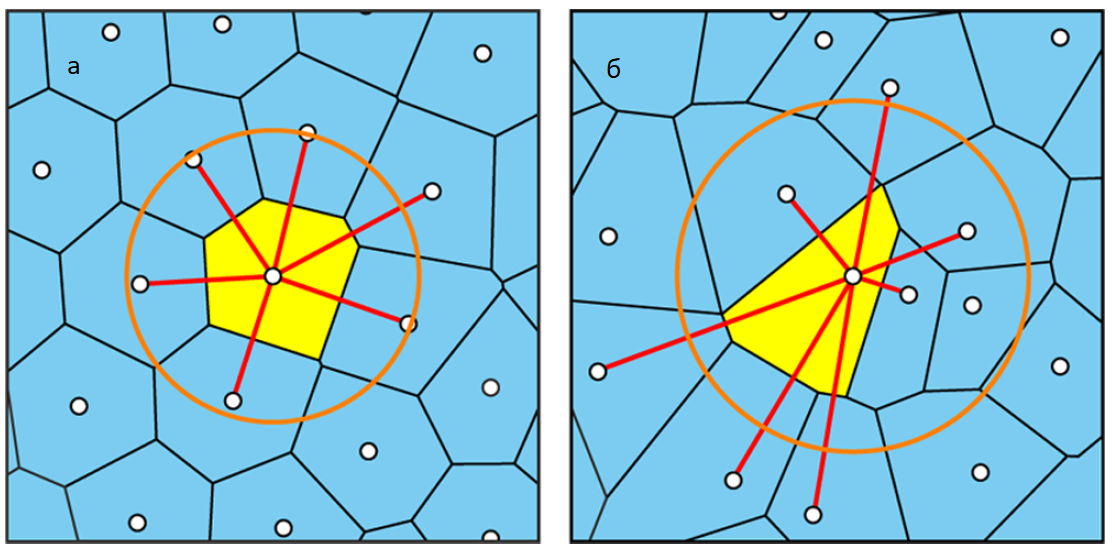
\includegraphics[width=0.7\textwidth]{rgcell}
\caption{Пример разбиения на ячейки вороного в конденсированном кластере (а) и газе (б). Частицы представлены белыми точками, а ячейки, соответствующие рассматриваемым частицам раскрашены в желтый цвет. Радиус окружностей соответствует среднему расстоянию между частицей и ее соседями.}
\label{risFlucMed}
\end{center}
\end{figure}

На рисунке \ref{risFlucMed} показана часть $2D$ - системы, полученной с использованием МД-моделирования потенциала Леннарда-Джонса (LJ12-6 при плотности частиц $n_0 = 0.4$).
Сравнивая ячейки вороного в конденсированной среде и газе можно заметить, что конденсированное состояние отличается меньшей площадью частиц. Из-за большей плотности частиц в конденсате, расположение частиц сильно ограниченно, вследствие чего ячейки получаются более правильной формы. Это дает возможность ввести некоторую величину, которая будет показывать отклонение от правильной формы.

\begin{equation}
	R_{0i} = \sqrt{\frac{\pi}{2 S_i N_{ni}^2} \sum\limits_{i<k}^{N_{ni}} (r_{ij} - r_{ik})^2}, r_{ij} = |r_i - r_j|,
\end{equation}

где $S_i$ - площадь рассматриваемой частицы, $N_{ni}$ - количество соседей частицы; $r_{ij}$ - расстояние от рассматриваемой частицы до соседней.
Для уменьшения сильных колебаний величины $R_{0i}$, она усредняется по соседним частицам:

\begin{equation}\label{eqIrreg}
R_i = \frac{1}{N_{ni} + 1} \left( R_{0i} + \sum\limits_{j=1}^{N_{ni}} R_{0j} \right),
\end{equation}

где $R_{0i}$ - неусредненный параметр искомой частицы, рассчитанный по формуле \ref{eqIrreg}; $R_{0j}$ - соответствующие параметры для соседних частиц.  
Далее данная величина будет называться \textbf{параметром иррегулярности}.

\begin{figure}[htbp!]
\begin{center}
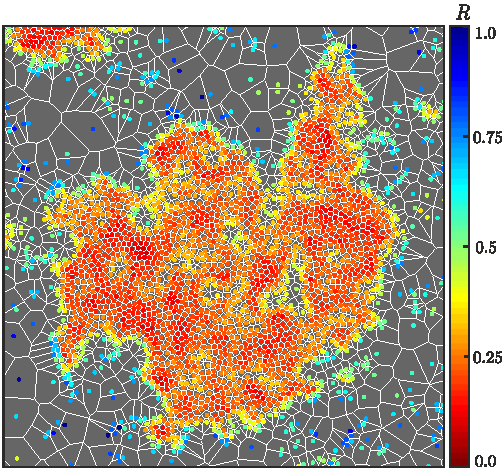
\includegraphics[width=0.7\textwidth]{MPI-Figure1}
\caption{Пример конденсированного кластера в системе с потенциалом Леннарда-Джонса. Ячейки вороного раскрашены в белый цвет, частицы раскрашены по величине параметра $R$.}
\label{risIrreg}
\end{center}
\end{figure}

На рисунке \ref{risIrreg} представлен конденсированный кластер, частицы которого раскрашены в соответствии с параметром иррегулярности. Чем он меньше, чем более упорядочена система. В идеальном кристалле данный параметр равен нулю.

Поскольку параметр $R$ мал для частиц принадлежащих кластерам конденсата, мы можем использовать следующее неравенство для их определения:

\begin{equation}
R < R_t,
\end{equation}

где $R_t$ - порог для частиц конденсата.
По причине больший флуктуаций величины $R$, кроме обрезки по параметру $R_t$, требуется корректировка фаз.

Корректировка фаз включает в себя следующие условия:

\begin{itemize}
\item частица конденсата, не имеющая среди своих соседей частиц того же типа, является поверхностью.
\item газовая частица, не имеющая соседних частиц того же класса,  является поверхностью.
\item частица конденсата, которая имеет среди соседних частиц, газовую частицу, является поверхностью.
\item частица поверхности, не имеющая среди соседей частиц газа, является конденсатом.
\item поверхностная частица, не имеющая среди соседей частиц конденсата, является газом.
\end{itemize}


\begin{figure}[htbp!]
\begin{center}
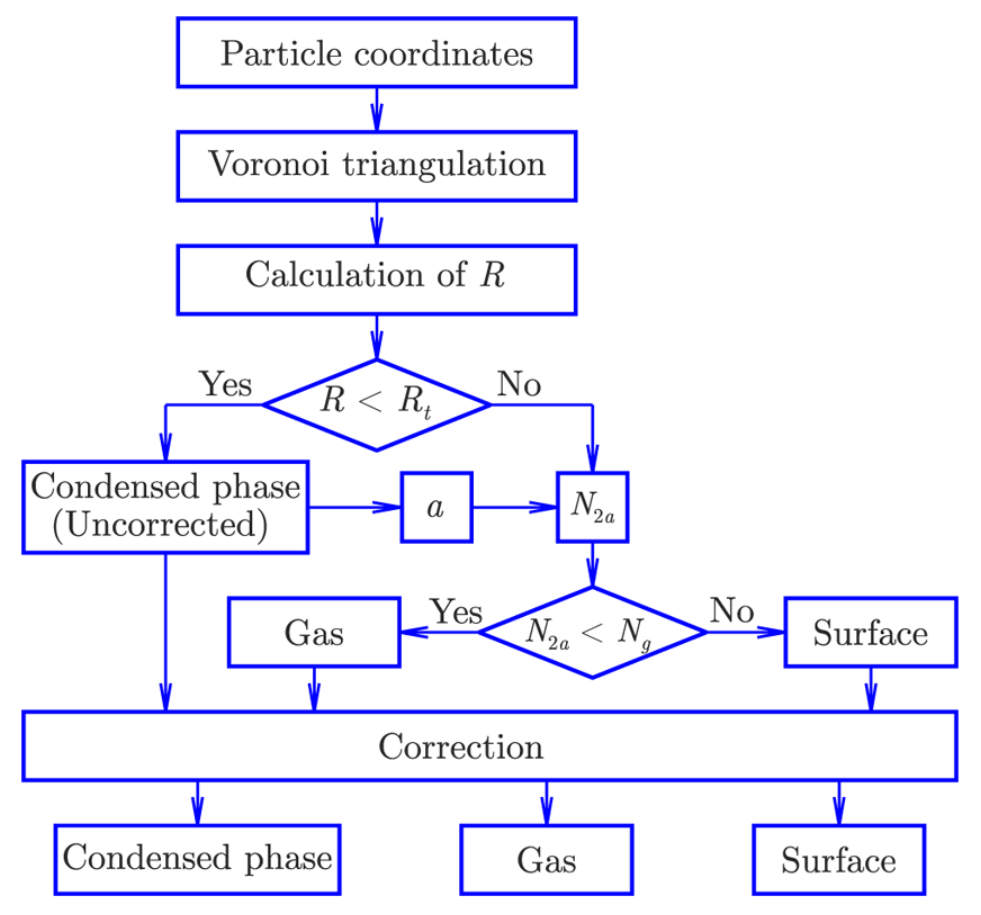
\includegraphics[width=0.5\textwidth]{shem_class}
\caption{Полная схема классификации частиц в системе.}
\label{risShemClass}
\end{center}
\end{figure}

Полная схема классификации частиц в системе, которая использует только координаты, представлена на рисунке \ref{risShemClass},
где $a$ - среднее расстояние между частицами; $N_g$ - некоторое пороговое значение для газовых частиц, находящихся на расстоянии $2a$ от выбранной частицы; $N_{2a}$ - число частиц, находящихся на расстоянии менее $2a$ от выбранной частицы. Если выполняется условие $N_{2a} < N_{g}$, то частица распознается как газ.
В данной работе константы приняты равными $R = 0.5, N_g = 5$.


По причине больший флуктуаций величины $R$, кроме обрезки по параметру $R_t$, требуется корректировка фаз.


Корректировка фаз включает в себя следующие условия:

\begin{itemize}
\item частица конденсата, не имеющая среди своих соседей частиц того же типа, является поверхностью.
\item частица конденсата, которая имеет среди соседних частиц, газовую частицу, является поверхностью.
\item газовая частица, не имеющая соседних частиц того же класса,  является поверхностью.
\item частица поверхности, все соседи которой принадлежат к классу "конденсат" или "газ", так же принадлежат к этому классу.
\end{itemize}

Данная корректировка повторяется несколько раз. Было установлено, что пяти раз достаточно, для приемлемого результата классификации.


\begin{figure}[htbp!]
\begin{center}
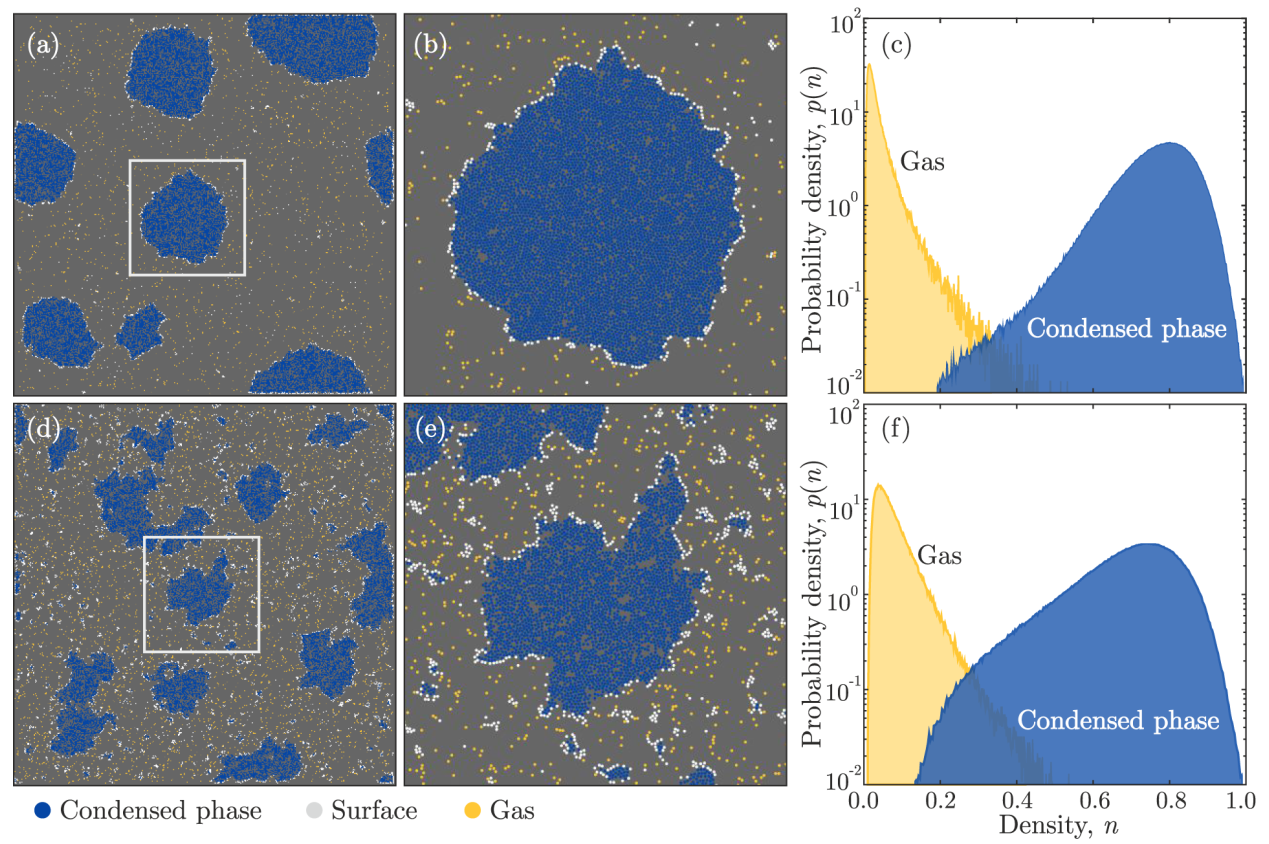
\includegraphics[width=0.8\textwidth]{articlePhaseAndDensity}
\caption{Слева - результат работы алгоритма, представленного на рисунке \ref{risShemClass}. Частицы разделены на 3 класса различными цветами: конденсат - синий, поверхность - белый, газ - желтый. Справа - плотность вероятности нахождения частицы газа и конденсата с данной плотностью.}
\label{risClassification}
\end{center}
\end{figure}

На рисунке \ref{risClassification} представлен результат классификации частиц в системе данным методом. Однако у данного алгоритма есть ряд недостатков. Так например возможны случаи распознавания пустот с газом внутри конденсированного кластера, как его часть, а также наблюдаются крупные скопления частиц поверхности, внутри который нет частиц, распознанных как конденсат.


После классификации всех частиц в системе и расчета плотностей по формуле \ref{eqRho}, возможно рассчитать мат. ожидание плотности конденсированных частиц и газа отдельно.
Рассчитав таким образом плотности при различных температурах, можно построить фазовую диаграмму в координатах $\rho, T$.


Однако прямой расчет плотности корректно работает только для конденсированных частиц, так как флуктуации размеров ячеек не велики, и на их размер не оказывают влияния частицы газа и поверхности. На площадь газовых частиц существенный эффект оказывают частицы поверхности, которые занимают сопоставимый объем, существенно увеличивая плотность первых.


В рамках данной работы был существенно переработан алгоритм корректировки фаз, который помимо условий представленных в оригинальной работе включает дополнительные условия:
\begin{itemize}
\item частица поверхности, не имеющая среди соседей частиц газа, является конденсатом.
\item поверхностная частица, не имеющая среди соседей частиц конденсата, является газом.

\item частицы конденсата, плотность которых сопоставима с плотностью поверхностных частиц, являются поверхностью. Данная проверка делается дважды (перед всеми остальными и после).

\item частица конденсата, которая имеет меньше 3 соседних частиц, так же принадлежащих к конденсату, является поверхностью.
\end{itemize}


Данные условия позволяют отделить крупные пустоты внутри кристалла от самого кристалла, и определить крупные скопления поверхностных частиц как небольшие кластеры конденсата или газ.


Так же был переработан алгоритм вычисления плотности газа в системе. Она вычисляется косвенно, по формуле:

\begin{equation}
\rho_{gas} = \frac{N_{g}}{S - (N_{b} + N_{c}) / \mathbb{M}\rho_c},
\label{eqGas}
\end{equation}

где $S$ - полная площадь, $N_g, N_b, N_c$ - число частиц газа, поверхности и конденсата соответственно; $\mathbb{M}\rho_c$ - мат. ожидание плотности частиц конденсата.

При данном подходе площадь поверхностных частиц считается равной плотности конденсата, что позволяет более объективно вычислять плотность газа.


\begin{figure}[htbp!]
\begin{center}
\includegraphics[width=0.7\textwidth]{Voronoi}
\caption{Разбиение на ячейки Вороного исследуемой системы на примере системы c потенциалом взаимодействия Леннарда-Джонса при различной температуре.}
\label{ris5}
\end{center}
\end{figure}

Текст

\begin{figure}[htbp!]
\begin{center}
\includegraphics[width=0.7\textwidth]{RG}
\caption{Параметр иррегулярности $R$ в исследуемой системы на примере системы c потенциалом взаимодействия Леннарда-Джонса при различной температуре.}
\label{ris6}
\end{center}
\end{figure}

Текст

\begin{figure}[htbp!]
\begin{center}
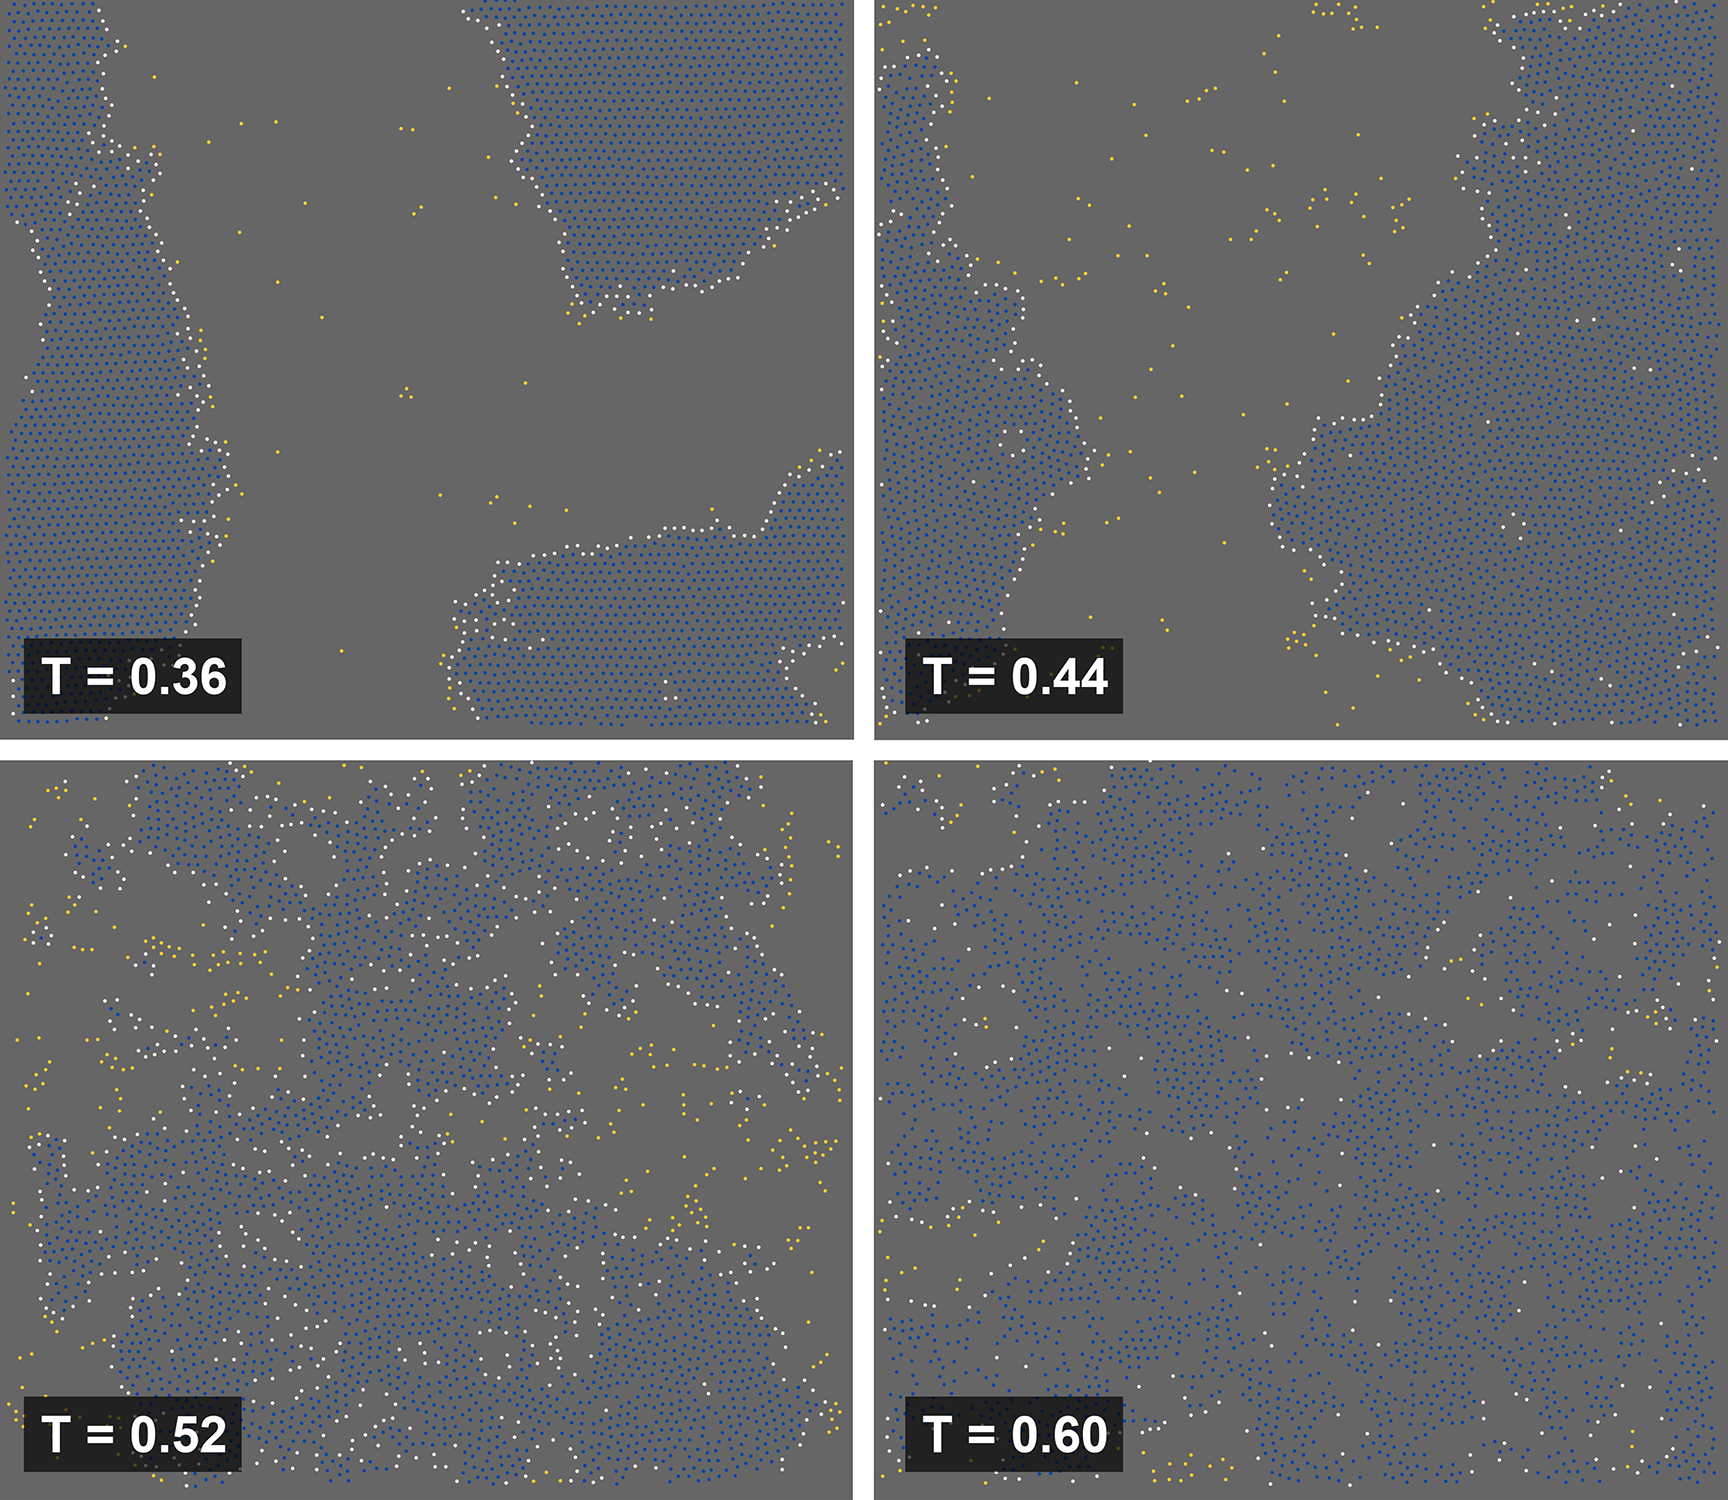
\includegraphics[width=0.7\textwidth]{classification}
\caption{Классификация частиц в исследуемой системы на примере системы c потенциалом взаимодействия Леннарда-Джонса при различной температуре.}
\label{ris7}
\end{center}
\end{figure}

Текст

\section{Построение фазовых диаграмм для различных потенциалов взаимодействия}\label{C2_2}

Текст

\begin{figure}[htbp!]
\begin{center}

\begin{minipage}[h]{0.45\linewidth}
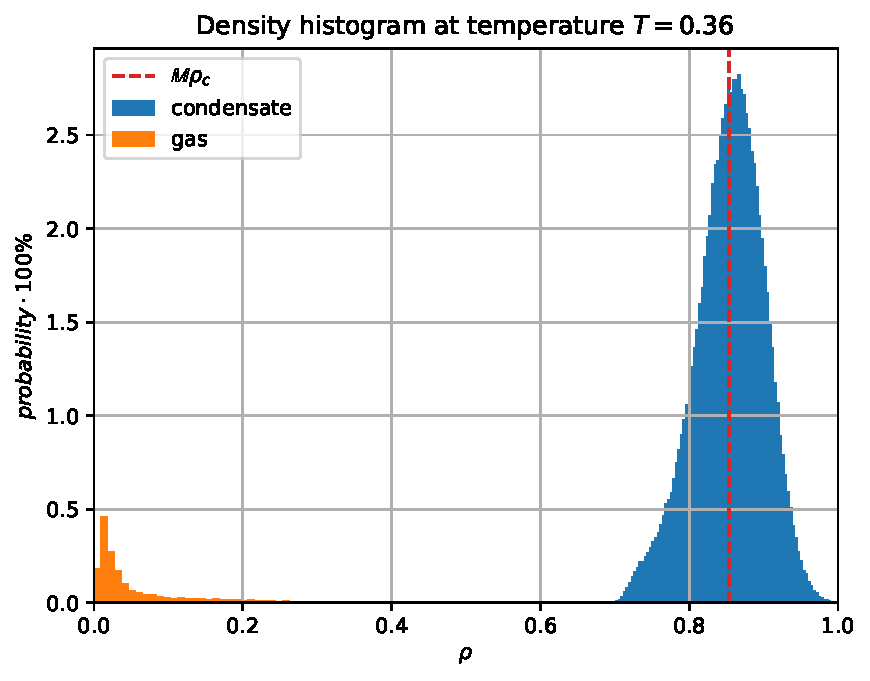
\includegraphics[width=\textwidth, keepaspectratio]{plot_hist_all_0.360}
\end{minipage}
%\hfill
\begin{minipage}[h]{0.45\linewidth}
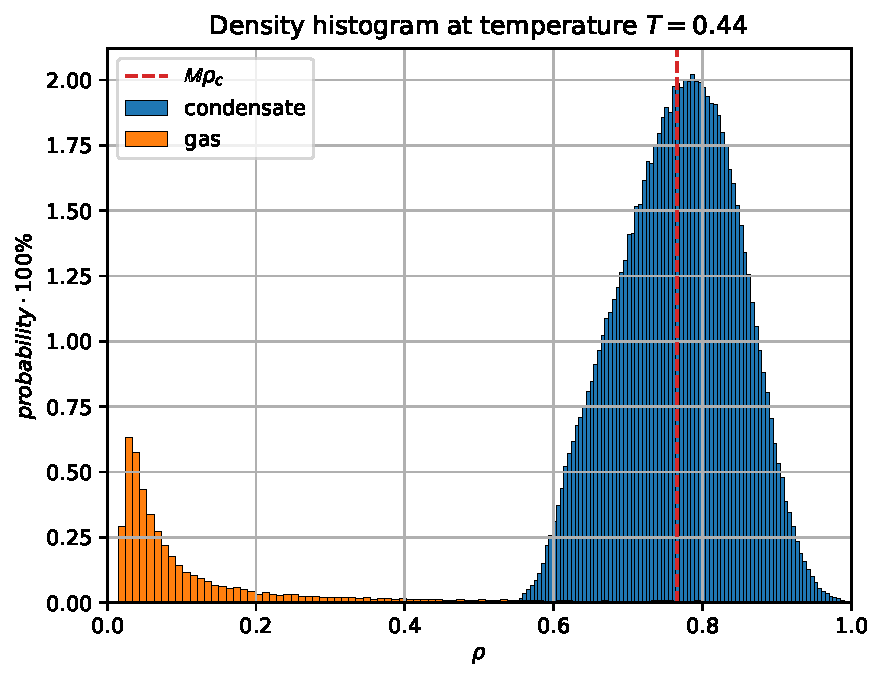
\includegraphics[width=\textwidth, keepaspectratio]{plot_hist_all_0.440}
\end{minipage}

%\vfill

\begin{minipage}[h]{0.45\linewidth}
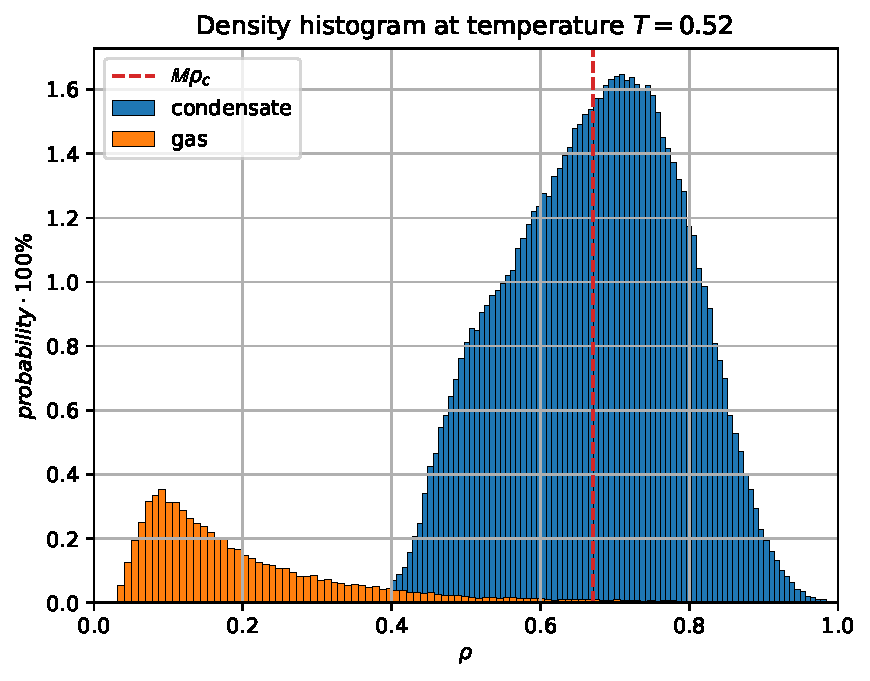
\includegraphics[width=\textwidth, keepaspectratio]{plot_hist_all_0.520}
\end{minipage}
%\hfill
\begin{minipage}[h]{0.45\linewidth}
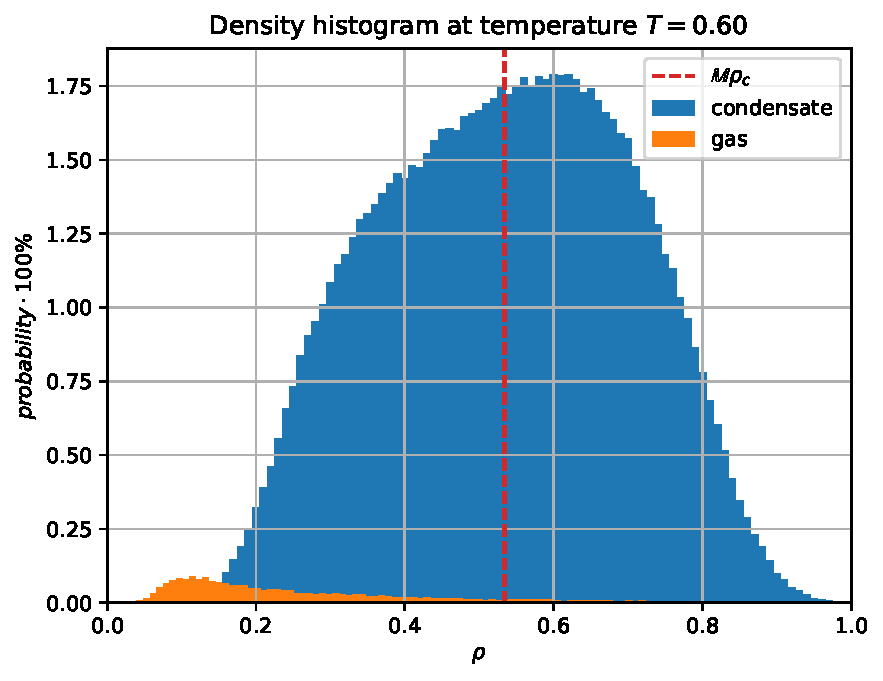
\includegraphics[width=\textwidth, keepaspectratio]{plot_hist_all_0.600}
\end{minipage}
\caption{Распределение плотностей частиц конденсата и газа при различных температурах. Красной вертикальной линией указано математическое ожидание плотности конденсатных частиц.}
\label{ris8}
\end{center}
\end{figure}


Текст


\begin{figure}[htbp!]
\begin{center}
\begin{minipage}[h]{0.45\linewidth}
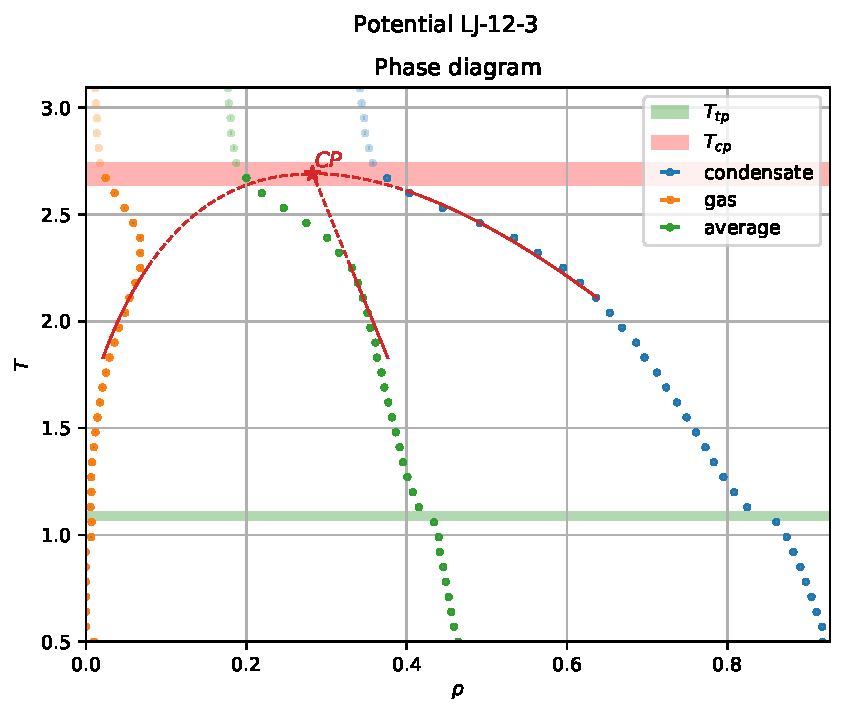
\includegraphics[width=\textwidth, keepaspectratio]{plot_phase_diagram_Potential LJ-12-3_1}
\end{minipage}
%\hfill
\begin{minipage}[h]{0.45\linewidth}
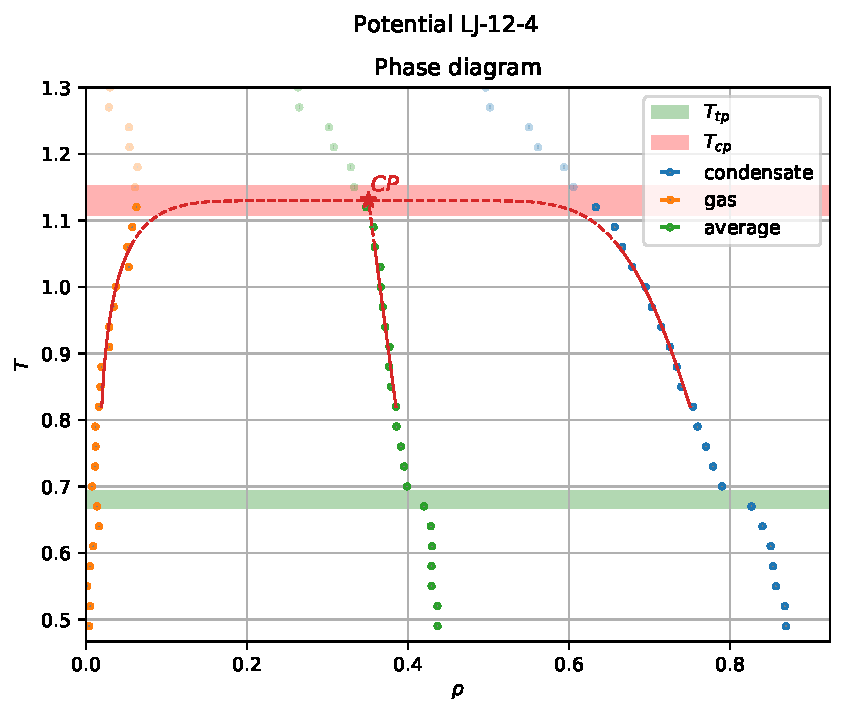
\includegraphics[width=\textwidth, keepaspectratio]{plot_phase_diagram_Potential LJ-12-4_1}
\end{minipage}

%\vfill

\begin{minipage}[h]{0.45\linewidth}
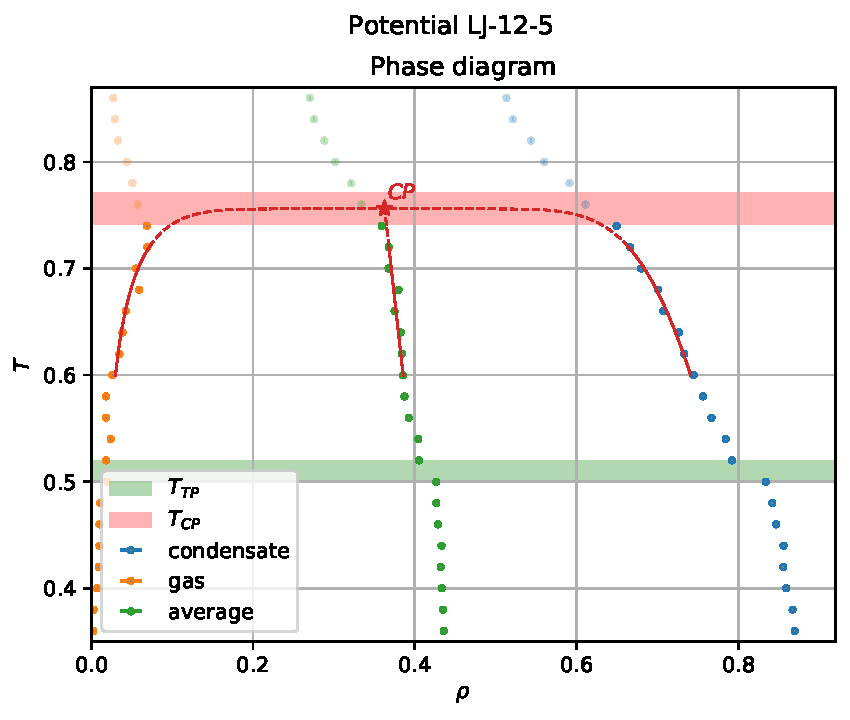
\includegraphics[width=\textwidth, keepaspectratio]{plot_phase_diagram_Potential LJ-12-5_1}
\end{minipage}
%\hfill
\begin{minipage}[h]{0.45\linewidth}
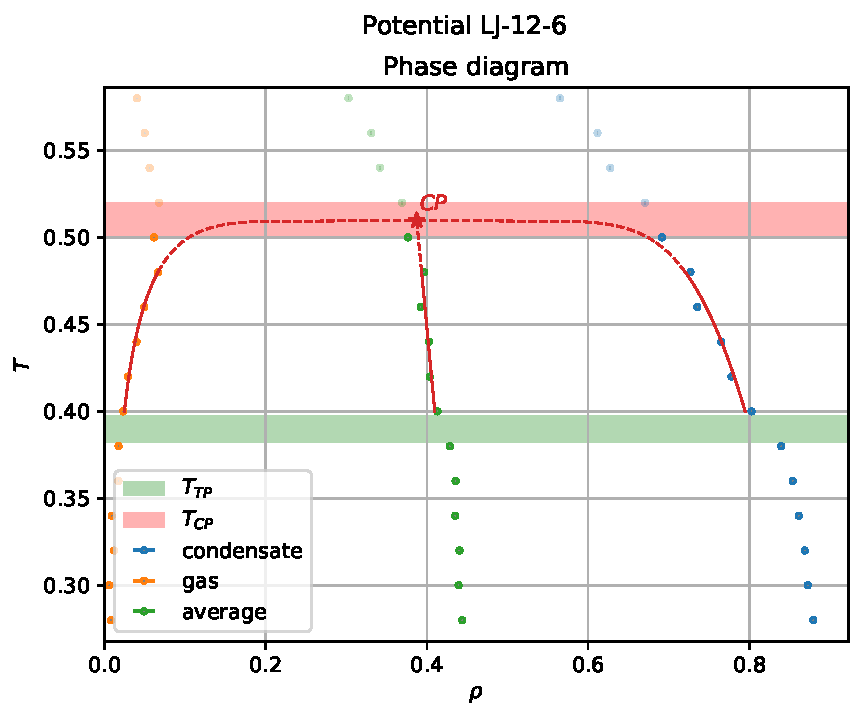
\includegraphics[width=\textwidth, keepaspectratio]{plot_phase_diagram_Potential LJ-12-6_1}
\end{minipage}
\caption{Фазовые диаграммы для систем с различными потенциалами взаимодействия.}
\label{ris9}
\end{center}
\end{figure}


Текст


\begin{figure}[htbp!]
\begin{center}
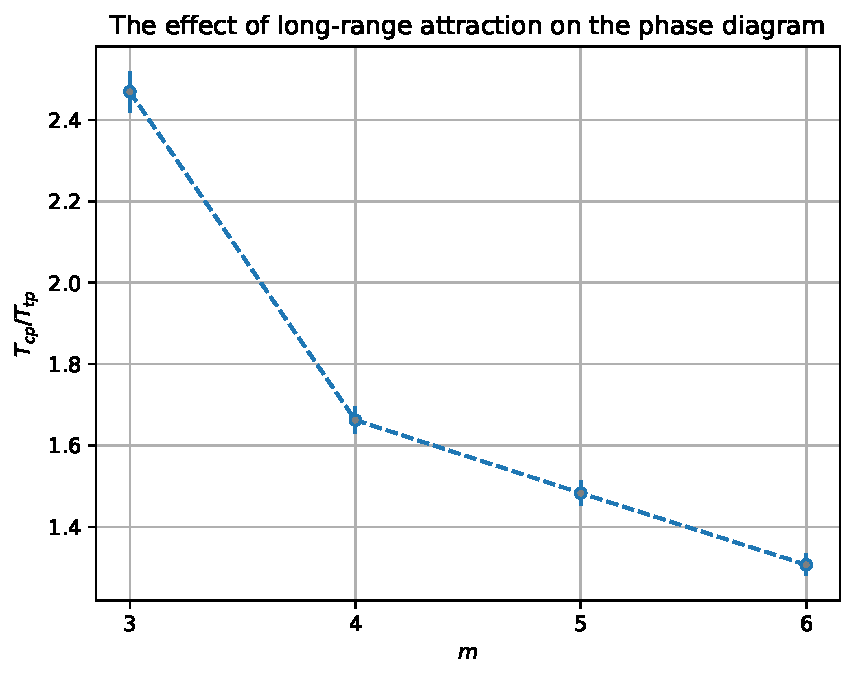
\includegraphics[width=0.7\textwidth]{effect of long-range attraction}
\caption{Отношение температур критической к тройной в зависимости от степени $m$ слагаемого в потенциале, отвечающего за притяжение.}
\label{ris10}
\end{center}
\end{figure}


\section{Анализ гистограмм распределения}\label{C2_3}

Текст

\begin{figure}[htbp!]
\begin{center}
\begin{minipage}[h]{0.45\linewidth}
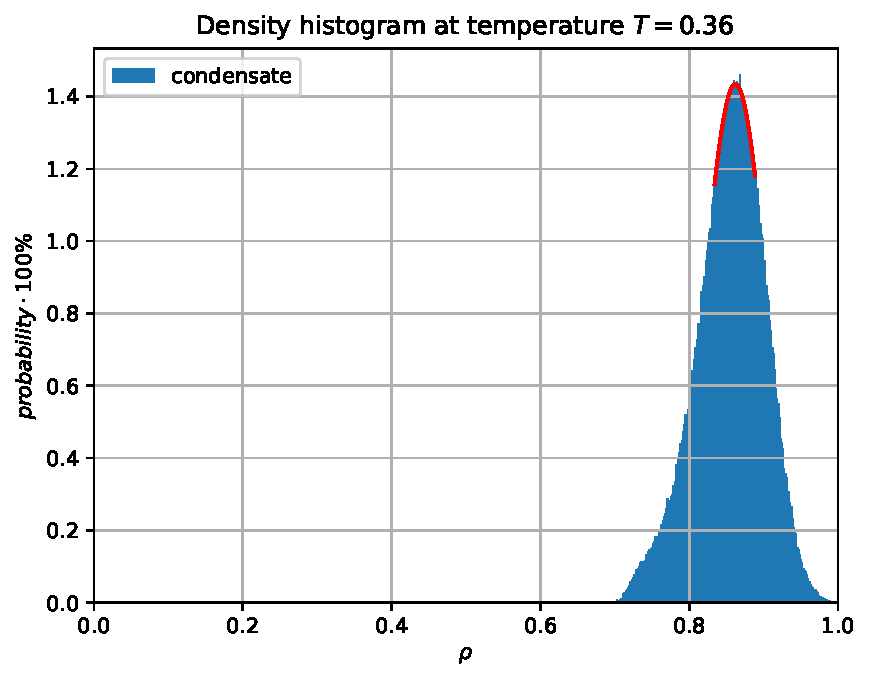
\includegraphics[width=\textwidth, keepaspectratio]{plot_hist_fit_0.360}
\end{minipage}
%\hfill
\begin{minipage}[h]{0.45\linewidth}
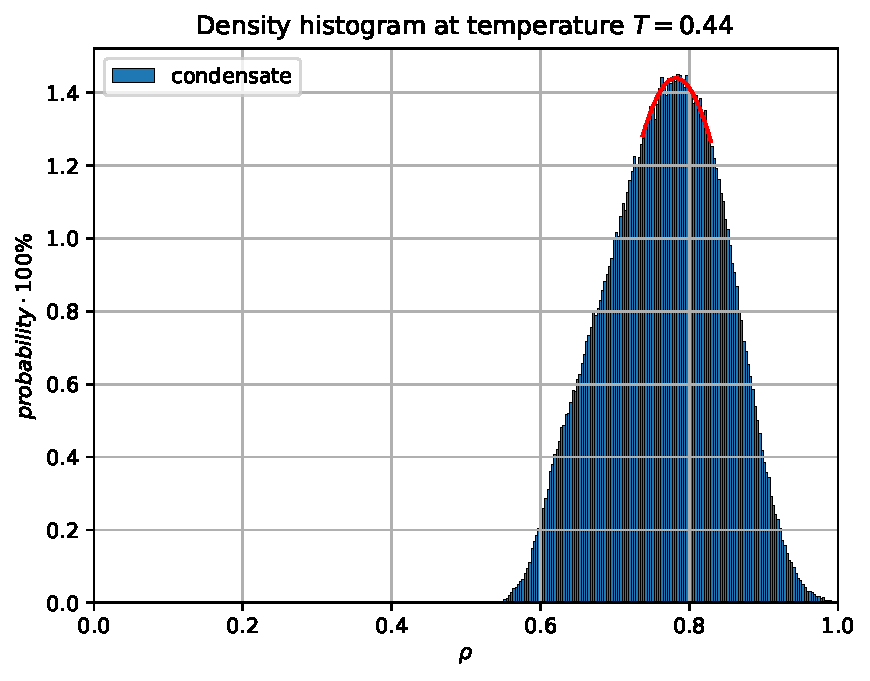
\includegraphics[width=\textwidth, keepaspectratio]{plot_hist_fit_0.440}
\end{minipage}

%\vfill

\begin{minipage}[h]{0.45\linewidth}
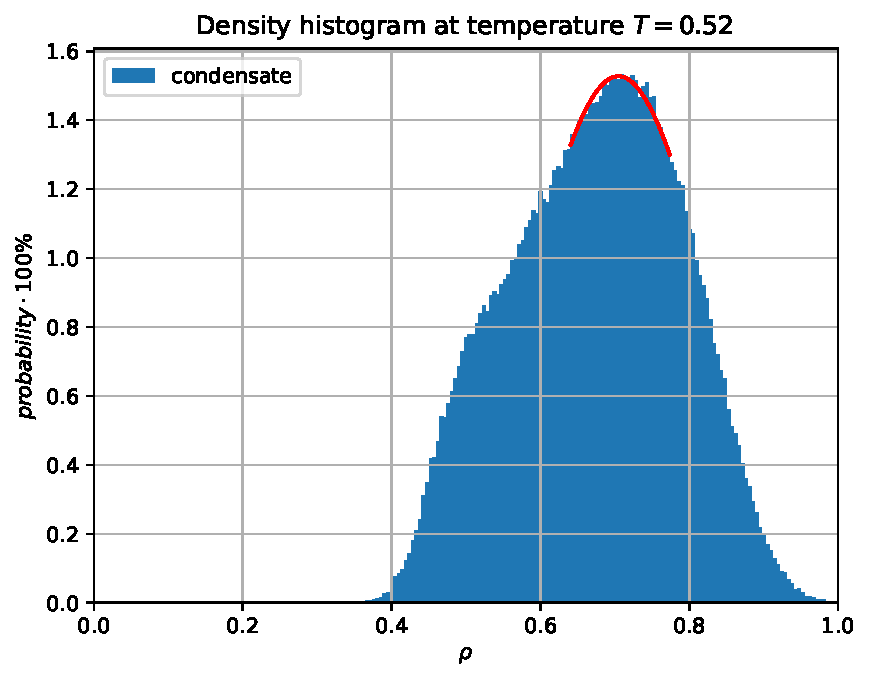
\includegraphics[width=\textwidth, keepaspectratio]{plot_hist_fit_0.520}
\end{minipage}
%\hfill
\begin{minipage}[h]{0.45\linewidth}
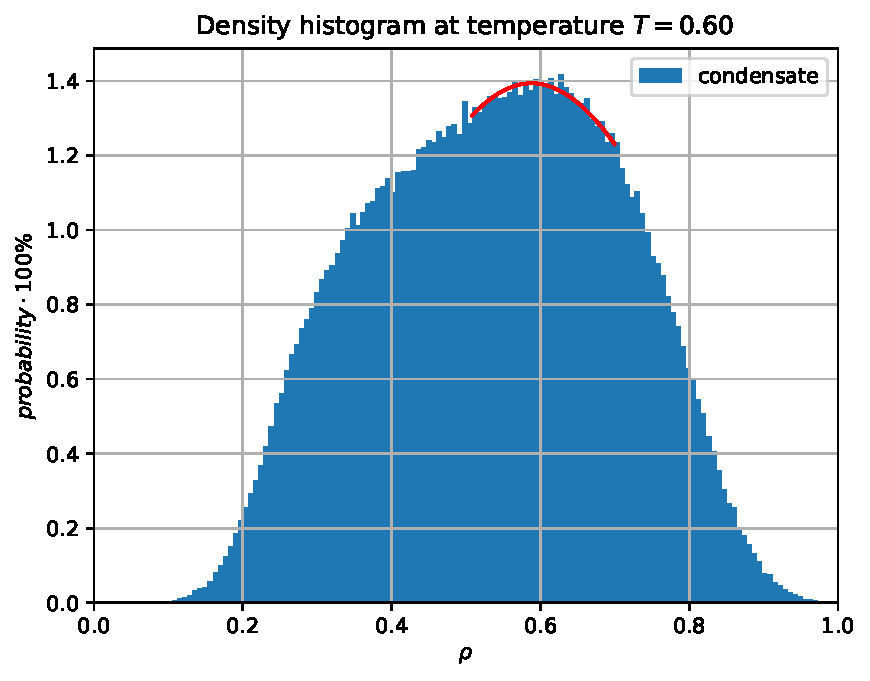
\includegraphics[width=\textwidth, keepaspectratio]{plot_hist_fit_0.600}
\end{minipage}
\caption{Аппроксимация пика распределения при различной температуре.}
\label{ris11}
\end{center}
\end{figure}

Текст

\begin{figure}[htbp!]
\begin{center}
\begin{minipage}[h]{0.45\linewidth}
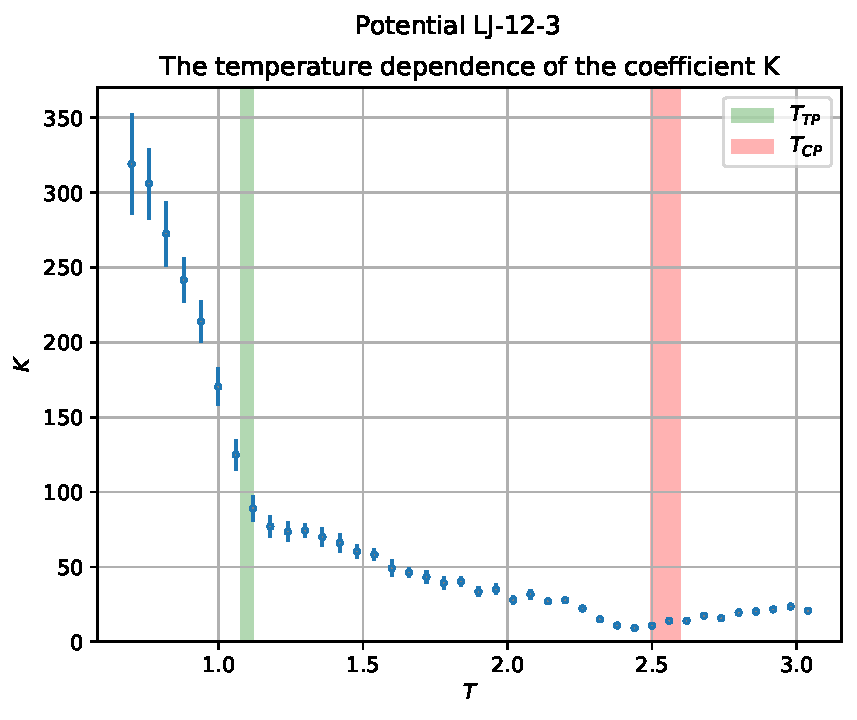
\includegraphics[width=\textwidth, keepaspectratio]{plot_K_Potential LJ-12-3_1}
\end{minipage}
%\hfill
\begin{minipage}[h]{0.45\linewidth}
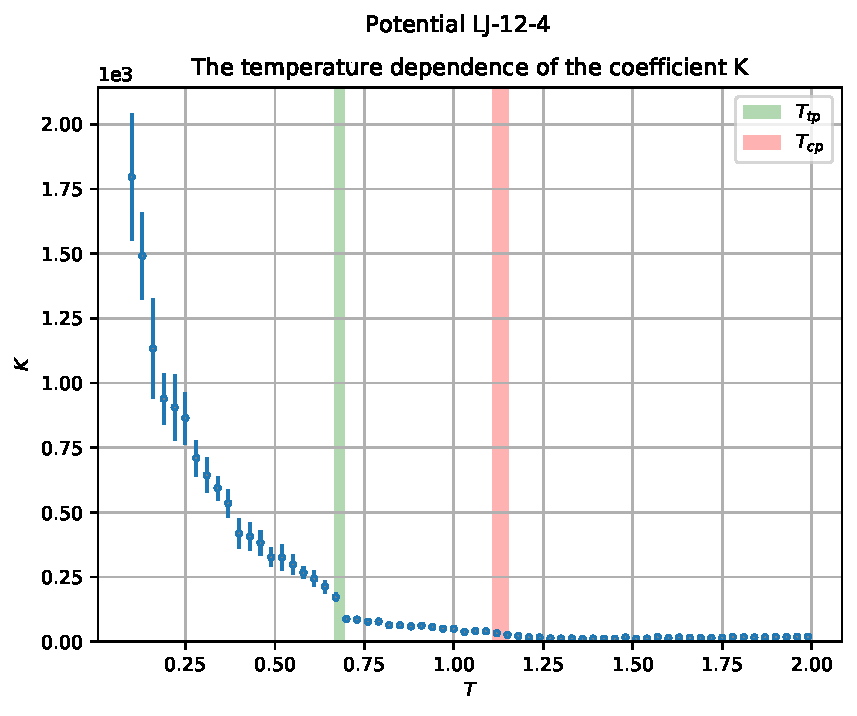
\includegraphics[width=\textwidth, keepaspectratio]{plot_K_Potential LJ-12-4_1}
\end{minipage}

%\vfill

\begin{minipage}[h]{0.45\linewidth}
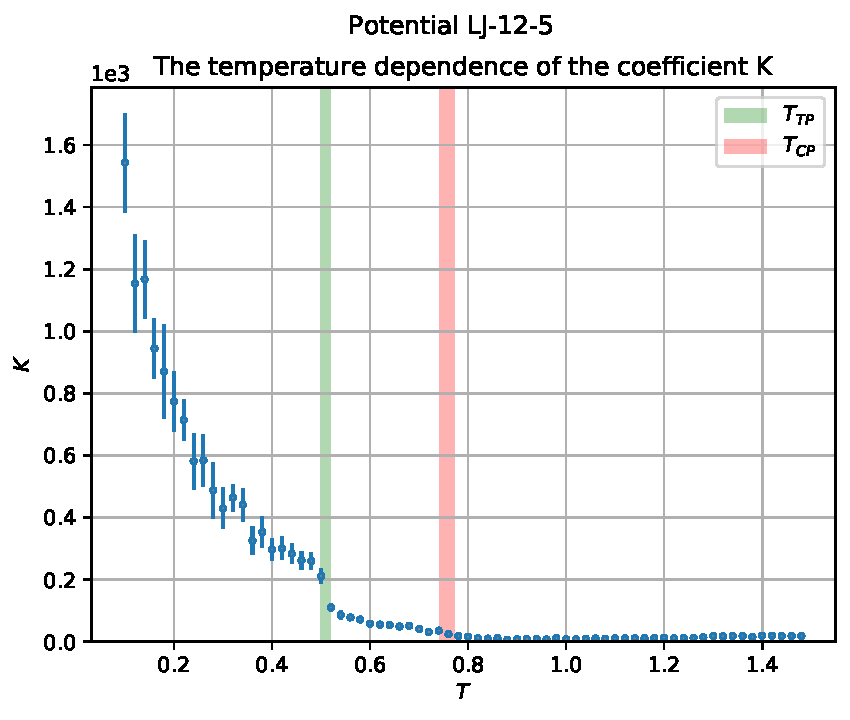
\includegraphics[width=\textwidth, keepaspectratio]{plot_K_Potential LJ-12-5_1}
\end{minipage}
%\hfill
\begin{minipage}[h]{0.45\linewidth}
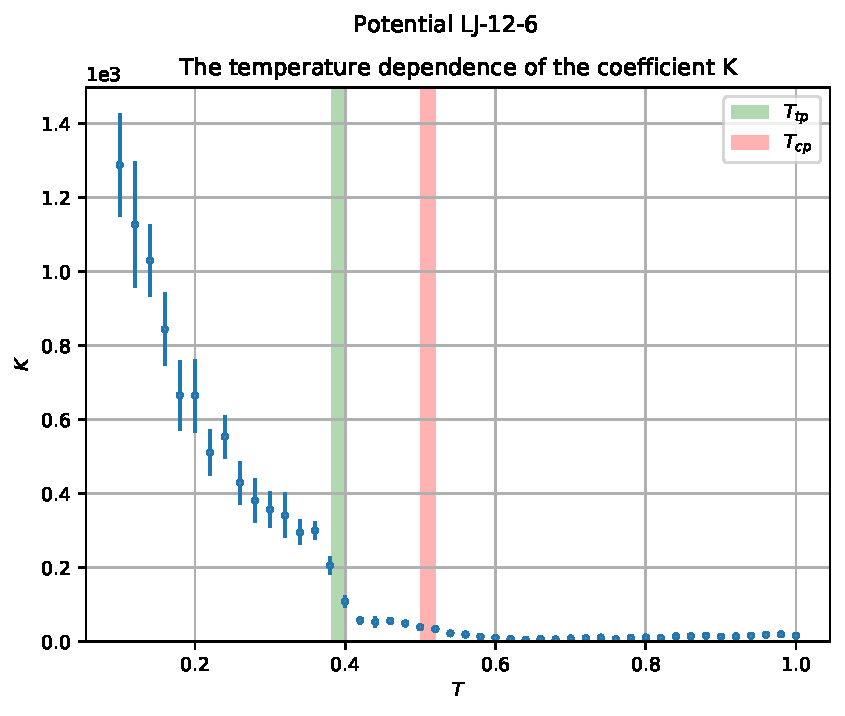
\includegraphics[width=\textwidth, keepaspectratio]{plot_K_Potential LJ-12-6_1}
\end{minipage}
\caption{Температурная зависимость коэффициента $K$.}
\label{ris12}
\end{center}
\end{figure}

Текст


\begin{figure}[htbp!]
\begin{center}
\begin{minipage}[h]{0.45\linewidth}
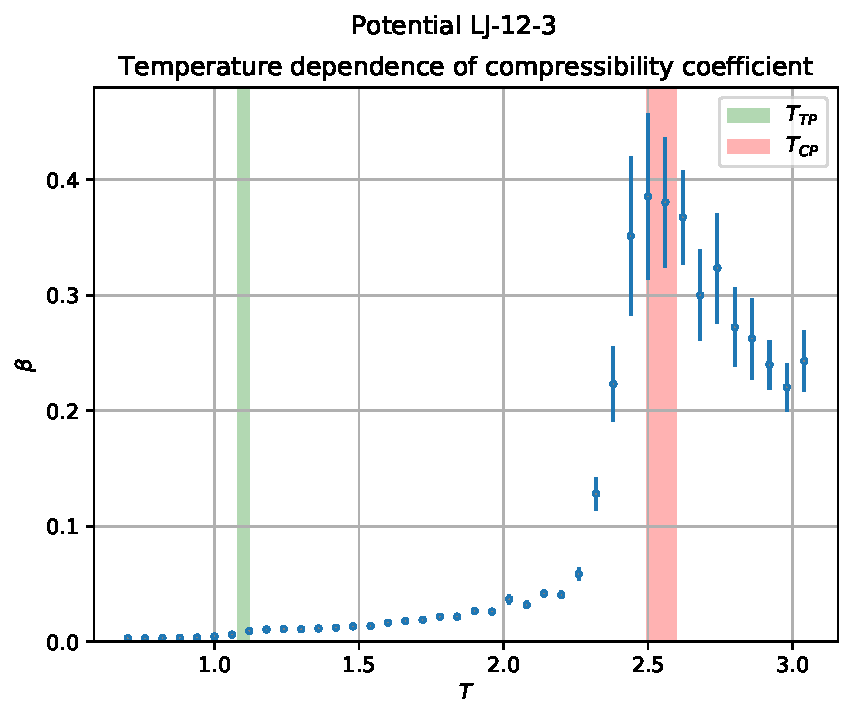
\includegraphics[width=\textwidth, keepaspectratio]{plot_compress_Potential LJ-12-3_1}
\end{minipage}
%\hfill
\begin{minipage}[h]{0.45\linewidth}
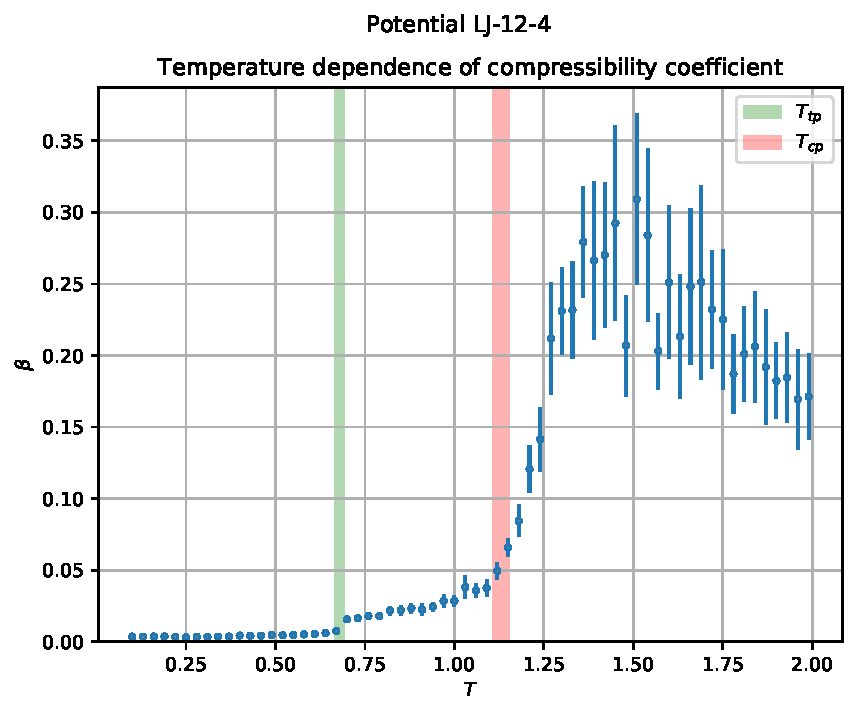
\includegraphics[width=\textwidth, keepaspectratio]{plot_compress_Potential LJ-12-4_1}
\end{minipage}

%\vfill

\begin{minipage}[h]{0.45\linewidth}
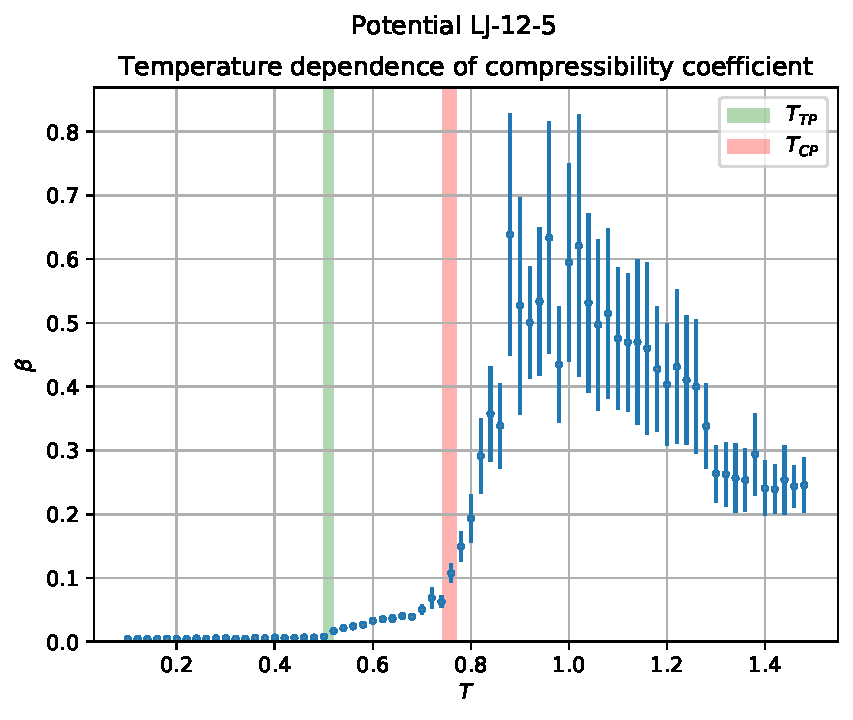
\includegraphics[width=\textwidth, keepaspectratio]{plot_compress_Potential LJ-12-5_1}
\end{minipage}
%\hfill
\begin{minipage}[h]{0.45\linewidth}
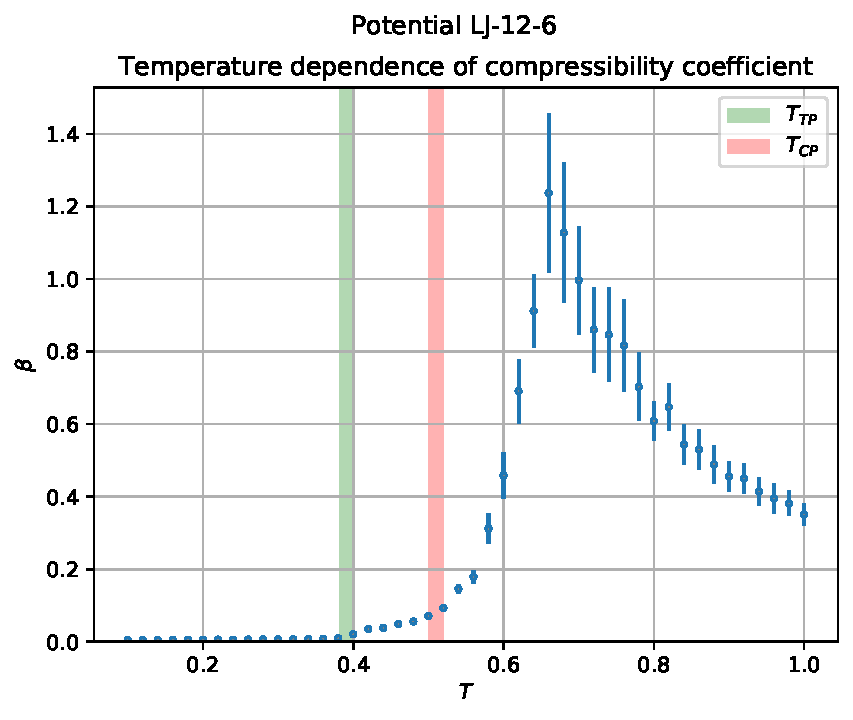
\includegraphics[width=\textwidth, keepaspectratio]{plot_compress_Potential LJ-12-6_1}
\end{minipage}
\caption{Температурная зависимость коэффициента $\beta$ сжимаемости вещества.}
\label{ris13}
\end{center}
\end{figure}

Текст

\begin{figure}[htbp!]
\begin{center}
\begin{minipage}[h]{0.45\linewidth}
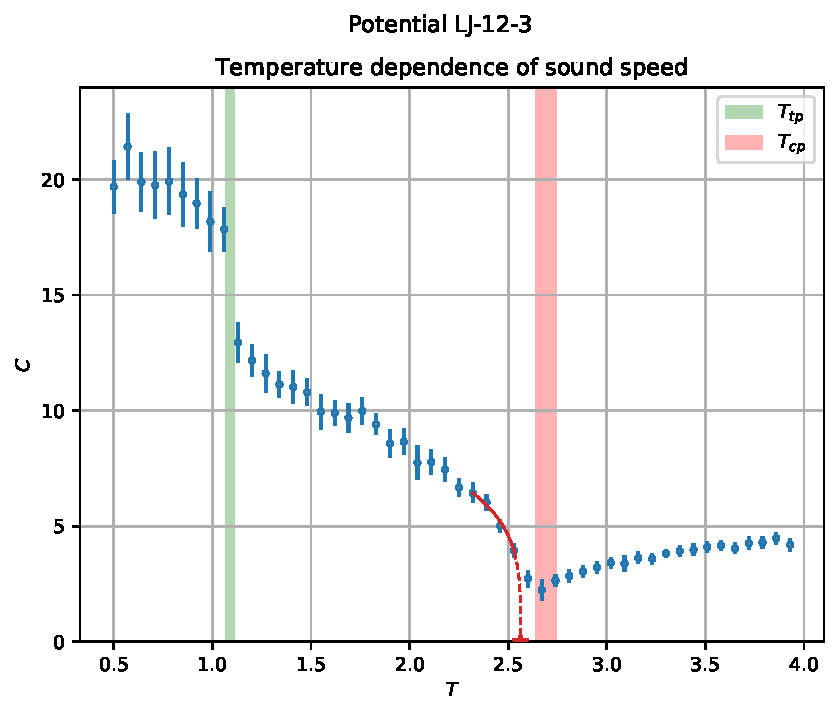
\includegraphics[width=\textwidth, keepaspectratio]{sound_speed_Potential LJ-12-3_1}
\end{minipage}
%\hfill
\begin{minipage}[h]{0.45\linewidth}
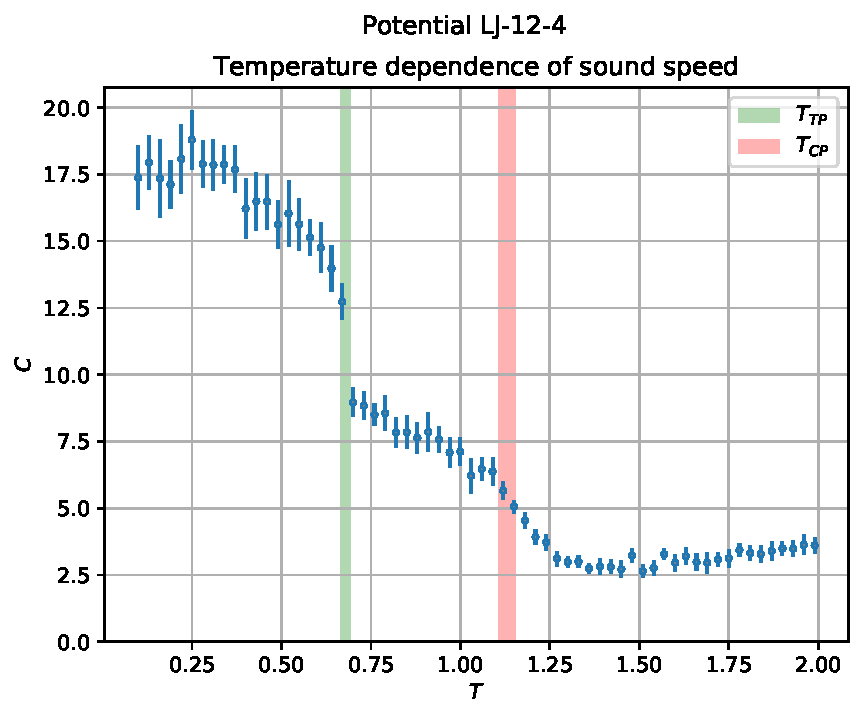
\includegraphics[width=\textwidth, keepaspectratio]{sound_speed_Potential LJ-12-4_1}
\end{minipage}

%\vfill

\begin{minipage}[h]{0.45\linewidth}
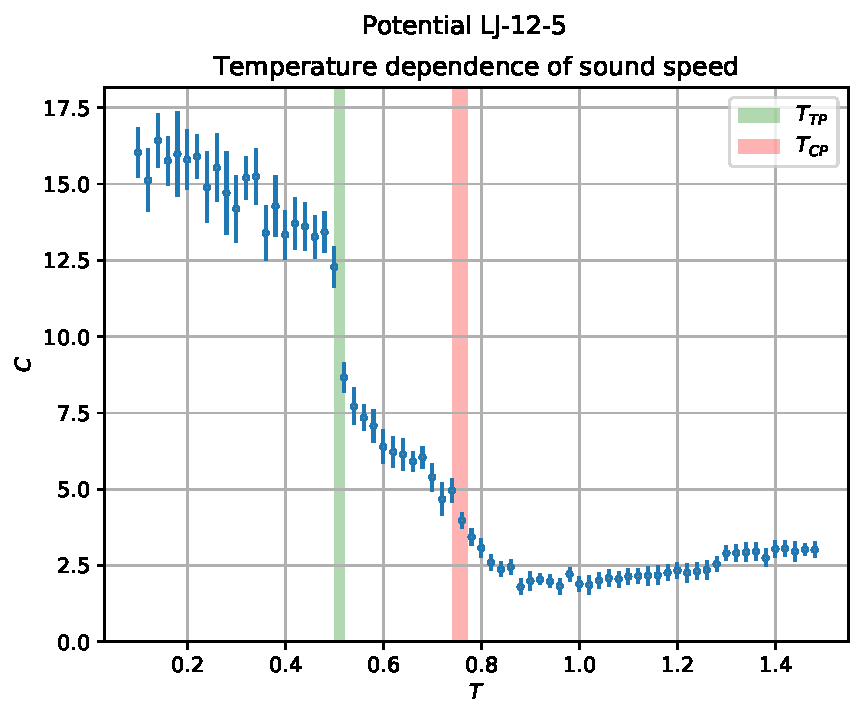
\includegraphics[width=\textwidth, keepaspectratio]{sound_speed_Potential LJ-12-5_1}
\end{minipage}
%\hfill
\begin{minipage}[h]{0.45\linewidth}
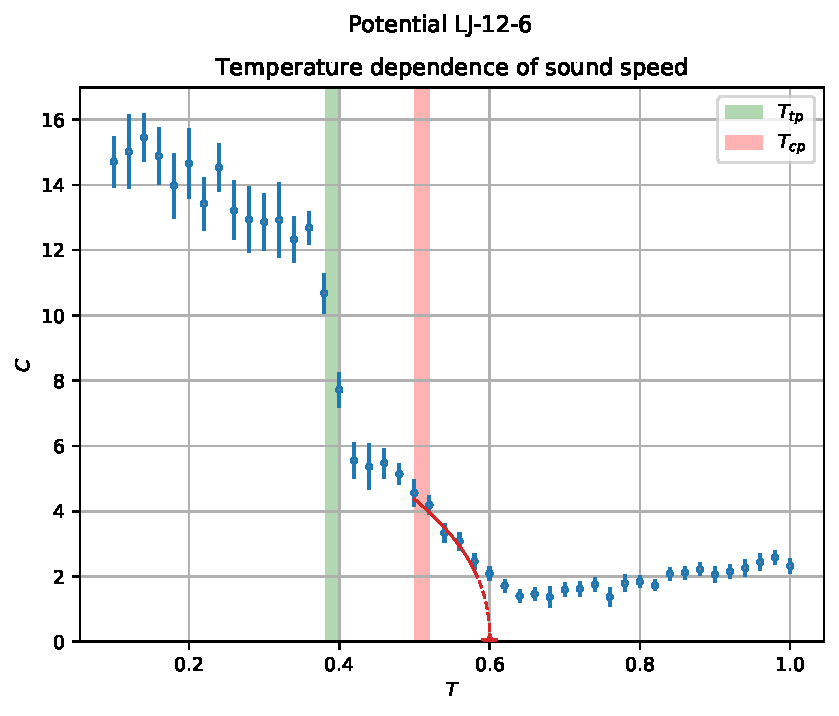
\includegraphics[width=\textwidth, keepaspectratio]{sound_speed_Potential LJ-12-6_1}
\end{minipage}
\caption{Температурная зависимость скорости звука в веществе.}
\label{ris14}
\end{center}
\end{figure}

Текст

\begin{figure}[htbp!]
\begin{center}
\begin{minipage}[h]{0.45\linewidth}
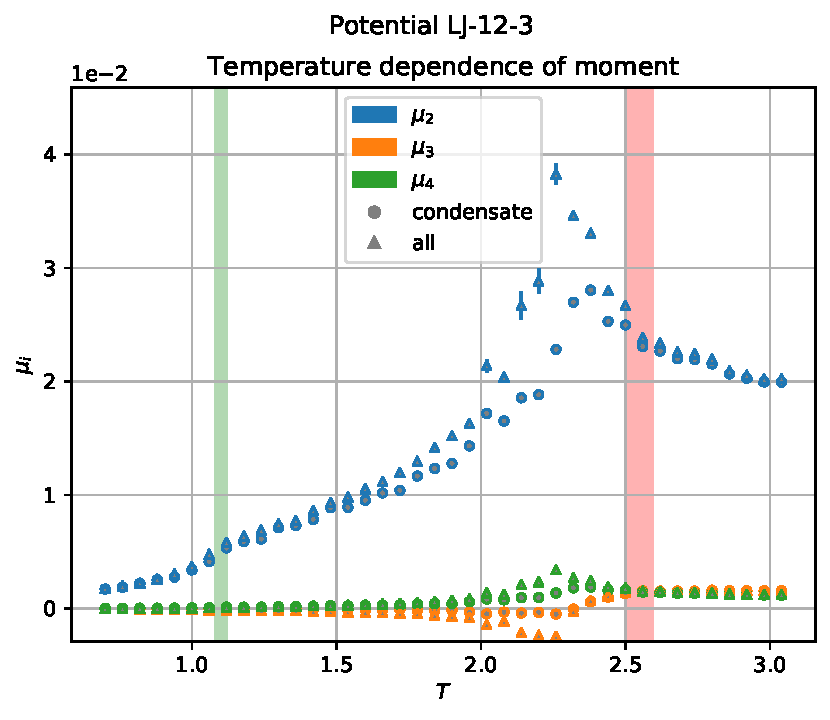
\includegraphics[width=\textwidth, keepaspectratio]{plot_moment_Potential LJ-12-3_1}
\end{minipage}
%\hfill
\begin{minipage}[h]{0.45\linewidth}
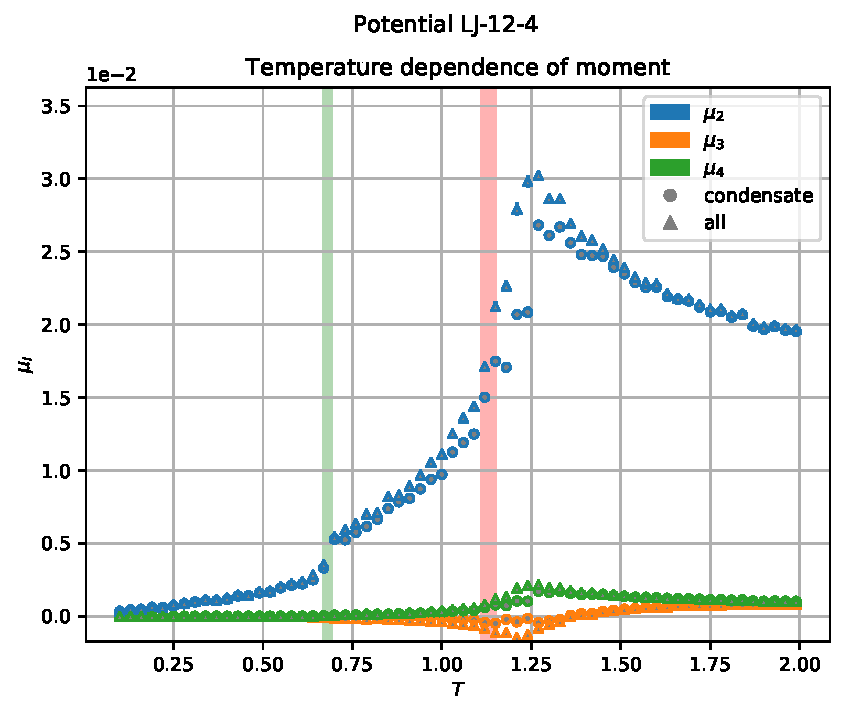
\includegraphics[width=\textwidth, keepaspectratio]{plot_moment_Potential LJ-12-4_1}
\end{minipage}

%\vfill

\begin{minipage}[h]{0.45\linewidth}
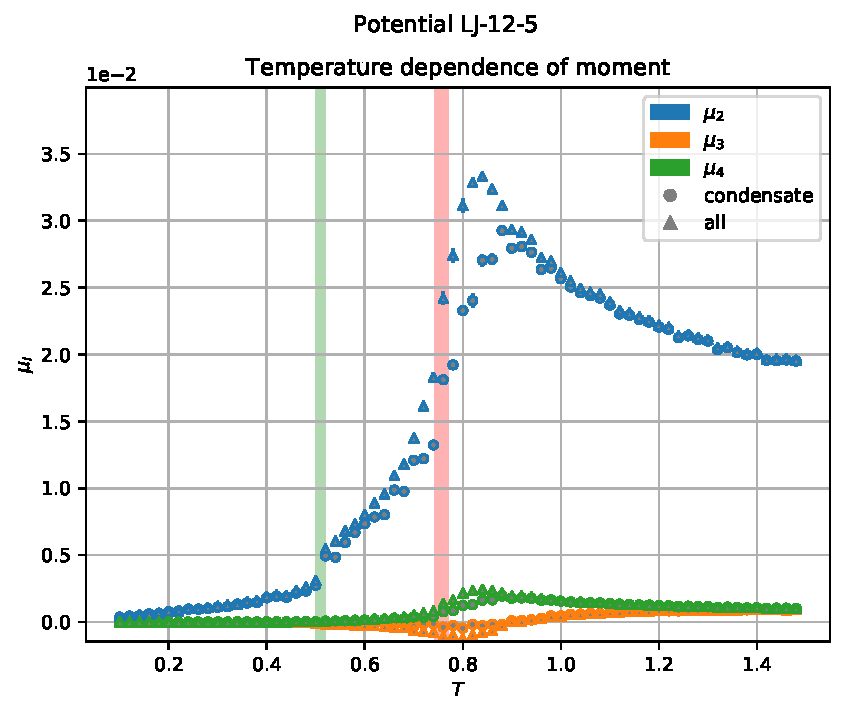
\includegraphics[width=\textwidth, keepaspectratio]{plot_moment_Potential LJ-12-5_1}
\end{minipage}
%\hfill
\begin{minipage}[h]{0.45\linewidth}
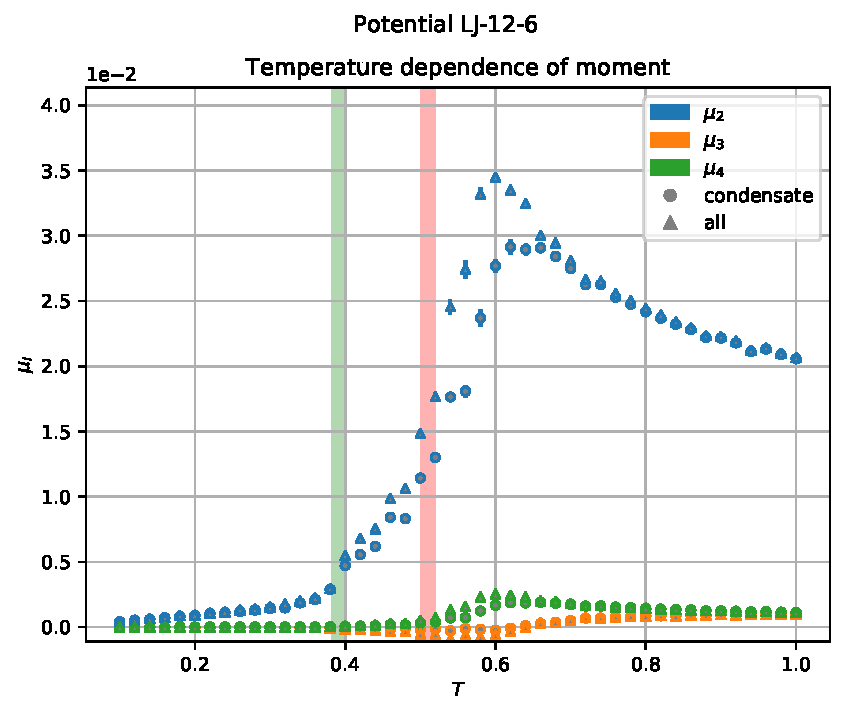
\includegraphics[width=\textwidth, keepaspectratio]{plot_moment_Potential LJ-12-6_1}
\end{minipage}
\caption{Температурная зависимость моментов величины $\mu$.}
\label{ris14}
\end{center}
\end{figure}

Текст

\section{Выводы главы}\label{C2_4}
Вывод.
